\chapter{Development of Testbench}
\label{ch:testbenchdevelop}
  
  The plan for developing Testbench4 was from two months to six weeks. This is
    a short period of time and to manage delivering a good-quality product you
    have to minimize overhead costs. We believe that a team should choose tools
    and methodology which suits its purposes. 
    Our team decided to use Scrum for managing product development and try to be agile and flexible.
    Our team consist of two developers and a product owner. And we decided to
    have two week sprints.

    \textbf{Scrum} is a management and control process that cuts through
    complexity to focus on building software that meets business needs. Management and teams are able to get their
    hands around the requirements and technologies, never let go, and deliver working software,
    incrementally and empirically. The Scrum Team consists of a Product Owner,
    the Development Team, and a Scrum Master.
    
  \textbf{Product Owner}(PO) - decides what features should the product have to
  maximally increase the satisfaction of the end user of the product and puts this features to the backlog.
  Backlog is a set of features in priority order.
  
  \textbf{Development team} - is
  a set of professionals that are working on implementing features of the product. 
  The team size should be from three to eight people. The team should work only on tasks from the backlog.
  
  \textbf{Scrum master} - a person who should help the team to increase their
  productivity by enhancing the understanding of teams strengths and weaknesses.

  The main idea of scrum is that development is done in short-time periods
  called sprints. Each spring consists of several phases:
  Sprint planning - when team decides what tasks should be done during the
  sprint .

  Main phase - when actual development is done.
  Sprint review - when team shows/demos the results to the product owner
  Retrospective - when team discuss what can be improved.


  Sprint may take from one to four weeks. The development team should decide
  what sprint length suits their needs. During sprint planning the team chooses
  which tasks will be moved from a product backlog to a sprint backlog.
  One of the restrictions is that the task in sprint backlog should be done in one sprint.
  If the team thinks that the task can not be finished in one sprint this task
  should be divided into several subtasks. 
  Having such one-sprint tasks helps the scrum team to keep track of the
  progress easily. Besides this gives an opportunity to receive feedback for each completed task at the end
  of the sprint. This helps to detect problems at the early stages, when
  the errors does not have a tremendous feedback. So even if a feature was misunderstood by the development team
  and you have to redone it completely , the team wastes time equal to the
  length of the spring at maximum. While in a classical waterfall model, a sequential design process in which
  progress is seen as flowing steadily through the phases of all development stages, 
  the error might be found much more lately, which will have a bigger negative impact.

  Another feature of Scrum is self organization of the team. The team should
  decide by itself which toolset to use. Tasks in scrum are not assigned to developers by a manager,
  but instead developers take items from the backlog by themselves.
  This approach saves time and reduces stress, because a person can pick a task,
  which he likes and understands. Developers pick tasks that they
  can finish before the end of the sprint.

  In our case we were not developing a new product, but releasing a new version.
  We didn’t find any arguments to change the tools were used in the previous release.

  \subsubsection {Tools used}
  
  \textbf{Maven}
  Maven is a java-based software project management and comprehension tool.
  Maven is based around the central concept of a build lifecycle. This means that the process for building 
  and distributing a particular project(artifact) is clearly defined. There are three built-in lifecycles:
  default, clean and site. Users can define their own lifecycle. Lifecycles consist of phases.
   
  The default lifecycle includes the following phases:
  \begin{itemize}
    \item validate - validate the project is correct and all necessary
    information is available.
    \item compile - compile the source code of the project.
    \item test - test the compiled source code using a suitable unit testing
    framework. These tests should not require the code be packaged or deployed
    package - take the compiled code and package it in its distributable format,
    such as a JAR.
    \item integration-test - process and deploy the package if necessary into an
    environment where integration tests can be run verify - run any checks to
    verify the package is valid and meets quality criteria
    \item install - install the package into the local repository, for use as a
      dependency in other projects locally.
    \item  deploy - done in an integration or
    release environment, copies the final package to the remote repository for
    sharing with other developers and projects.
  \end{itemize}
  
  The lifecycle phases are executed sequentially, in the example above if running maven deploy 
  all the phases will be executed. All maven configurations are specified in the Project Object Model (POM) file.
  POM is an XML file that contains information about the project and configuration details used by Maven 
  to build the project. 

  Maven reduces the complexity of developing and maintaining big projects.
  Nowadays applications may depend on dozens of third-party libraries and
  frameworks. Managing those dependencies manually is very time consuming. You
  need to find and download the exact version of the library and add it to your project build path.
  The libraries might have new versions you want to use, so you need to keep track of the versions
  of the dependencies and the versions of your application, because the might be incompatible. 
  You may want to have different configurations of your application for development and production or testing.
  And all the members of your team may have same or different configurations.
  Eventually, the complexity of managing your system will grow extremely. Maven helps to solve it.

  For example to define dependencies you define a dependency section in your POM file:
  \lstset{language=XML}
    \begin{lstlisting}
      <dependency>
         <groupId>group-a</groupId>
         <artifactId>artifact-b</artifactId>
         <version>1.0</version>
      </dependency>
    \end{lstlisting}  

  Afterwards all you team members will have the same dependency downloaded and
  added to your project. If you want to have different configurations for
  development and production you can specify the profile in your POM.
   \lstset{language=XML}
    \begin{lstlisting}
      <profile>
         <id>test</id>
         <activation>
            <property>
               <name>env</name>
               <value>test</value>
            </property>
         </activation>
      </profile>
    \end{lstlisting}
  Afterwards you can pass the profile name to the maven build phase as
  a parameter.

  Eventually, you have a set of predefined configurations for your application
  for the whole team. So any developer can checkout pom file from the repository
  call mvn deploy and he will have the same version of the application with all
  the specified parameters and downloaded dependencies. If you want to update
  your dependencies or you found an error in the pom file after you fix the
  problem, all your team members have to just checkout the new version of POM.
 
  \textbf{Trac}
  Trac is an enhanced wiki and issue tracking system for software development
  projects. Trac may include several projects and users or developers can
  create tasks (also called tickets) for these projects. The tickets may have different types:
  “new feature”, “enchantment”, “error/bug”. At the beginning of the project the product owner
  goes through the list of the tickets and add them to a new milestone.
  Milestone is a plan for the next release, which includes set of tickets.

  Tickets have different value for the end user, but developers can not always
  assess that value by themselves. Product owner should help the development team to figure out the
  value of each ticket for the end user. Based on the value and time estimation each ticket should be prioritized.
  Prioritizing tickets is a very important task and should be done as soon as
  possible, preferable before coding starts. This gives a clear vision for all
  members of the team what should be done.

  In the Testbench4 project we used the trac milestone as a product backlog. On
  the sprint planning we estimate which tasks can be completed at the end of the sprint 
  and move them to the sprint backlog. As sprint backlog we used a scrum board.
  Scrum board is a white board, divided into several sections for example “to be done”, “in progress”, “in review”,
  “closed”. Paper stickers represent tickets and the person who is working on
  the ticket. The workflow is the following - a developer picks the
  ticket from the sprint backlog queue called “to be done” 
  writes his name on the sticker and move it to the “in progress” section.
  After he submitted a patch to the code review he moves the sticker to another
  section and so on.
  
  Looking to the scrum board gives you a brief summary of every team member tasks and 
  also the current sprint progress. One can also find more detailed information
  about tickets and the project progress in Trac.
 
  
  As a version control system we used \textbf{Git} - distributed revision control system
  which focuses on speed, data integrity, and support for distributed,
  non-linear workflows. There are two types of revision control systems :
  
   \begin{itemize}
   \item Client-server - such version control systems as SVN and CVS, have a 
    a centralised model, where there's a copy of the current code on a central
    server, which users check out in order to work on locally. When a user made
    some changes, he updates from the central version (in case other people have
    made changes in the meantime), solve conflicts (same part of code was
    changed by different people at the same time) that might have arisen, and
    then push their code into the server. Afterwards other people can check it out again.

   \item Distributed revision control systems such as Git, are structured on a
    peer-to-peer basis: instead of one centralised repository. Every developer
    has their own repository and there is no main repository as in client-server
    control systems, all repositories are “equal”. Though in practise developers
    create a “master” repository, where everyone push their own changes and pull
    changes made by other developers.
  \end{itemize}
  
  One of the biggest advantage of distributed systems is that repositories are
  synchronised by exchanging change-sets in the form of patches, meaning that 
  only changes are sent. In systems like SVN every time you pull changes from
  the central repository you are downloading the whole snapshot of your application sources.
  
  Also Git lets developers to have their local history of changes and commits,
  but then when pushing changes to the master repository they can rebase these changes as one commit.
  This helps on one hand keep a local history of intermediate steps for
  developer, but on the other hand have only commits for completed changes/features in the main repository
  seen for all other developers. Git has a powerful set of tools including unix commands,
  for example to find all commits made by one person you can use log command and pipeline it to a grep 
  (print lines matching a pattern) command.
  
   Git-blame command allows you to see the history of every line of your source
   code. This is very useful, if you have questions about some particular few lines of code.
   You can find an author of those lines and ask him a question.
   
   Git-bisect command - is a binary search against revision graph, which helps to find the commit which
   introduced a bug.

  \textbf{Teamcity} - is a web-based build management and continuous integration
  tool. Teamcity allows running multiple builds and tests under different platforms and environments.
  Teamcity build combines maven, ant builds, git command and bash scripts.
  
  Teamcity builds may be started automatically or manually. One option is to create a configuration to run all
  tests every night or to setup running tests on every git commit. Teamcity
  provides also build dependencies, which can be very helpful if your project
  depends on some other projects or libraries, teamcity will first build all the dependencies and then run your build.
  
  During the development cycle we used four different configurations.
  \begin{itemize}
  \item Running tests on every git commit. This configuration is started when Gerrit patch is submitted.
   Running all tests for all browsers is very time consuming and may take several hours. 
   That is why in this configuration includes only JUnit tests and PhantomJS
   tests, which does not need to run the actual browser. These kind of tests show common errors for all browsers.
   Running those tests gives a developer a fast feedback, if his changes caused some problems.
   \item Running all tests on latest commit every night. This build triggers at
    specific time every night, when servers load is lower than during the day.
    This configuration includes all the heavy tests for specific browsers. All
    the tests are run on Google Chrome, Mozilla Firefox and Internet Explorer 8, 9, 10 and 11. 
    For every test suite teamcity will run the specific browser on a test
    cluster. Running such tests is very resource consuming, but provides a
    confidence that the application is supported by all browsers.
    \item Snapshot build is run every night. This build publishes the latest
    version of the product to a maven repository.  Users can download
    the snapshot build with the latest version of the product, if they want to
    test new features, but do not want to wait for the release build.
    \item Release build is run when the team releases a new version of the
    product. This includes building all the dependencies, running all the tests,
    specifying the version of the product, creating release notes, making tag in
    the Git repository, publishing a new version to maven repository and Vaadin
    website.
   \end{itemize}

\textbf{Gerrit} is a web-based code collaboration tool. Gerrit allows developers to
  review patches made by other developers. Gerrit has a very easy system of evaluating patches:
  \begin{itemize}
  \item -2 (veto) - patch has major problems.
  \item -1 (disapprove) - patch has minor problems.
  \item +1 (approve) - no problems found.
  \item +2 (approve) - can be pushed to master.
  \end{itemize}
  
  The difference between +1 and +2 is that the patch can not be pushed to git
  repository without having +2. The reviewer can give +1 if he is not sure about his level of competence
  and want someone else to inspect the patch. There are might be several configurations of the review process,
  Figure 1 shows the process used in the Testbench4 project.

  Firstly, a developer submits his changes(patch) to Gerrit. Gerrit triggers the
  specific build in Teamcity. This build includes building the project and
  running tests. After this step is finished, teamcity returns a report about the build, if there are problems 
  the report is send to the developer and the patch is marked as -2. If all
  tests pass gerrit marks the patch as ready for review and put it to the list of waiting for review patches.
  Then the reviewer evaluates the patch. Given the patch -1 or -2 means that the developer should fix the problems,
  and submit the next version of the patch. The process continues until someone
  marks the patch as +2,  meaning in can be pushed to git master repository.
    \begin{figure}
      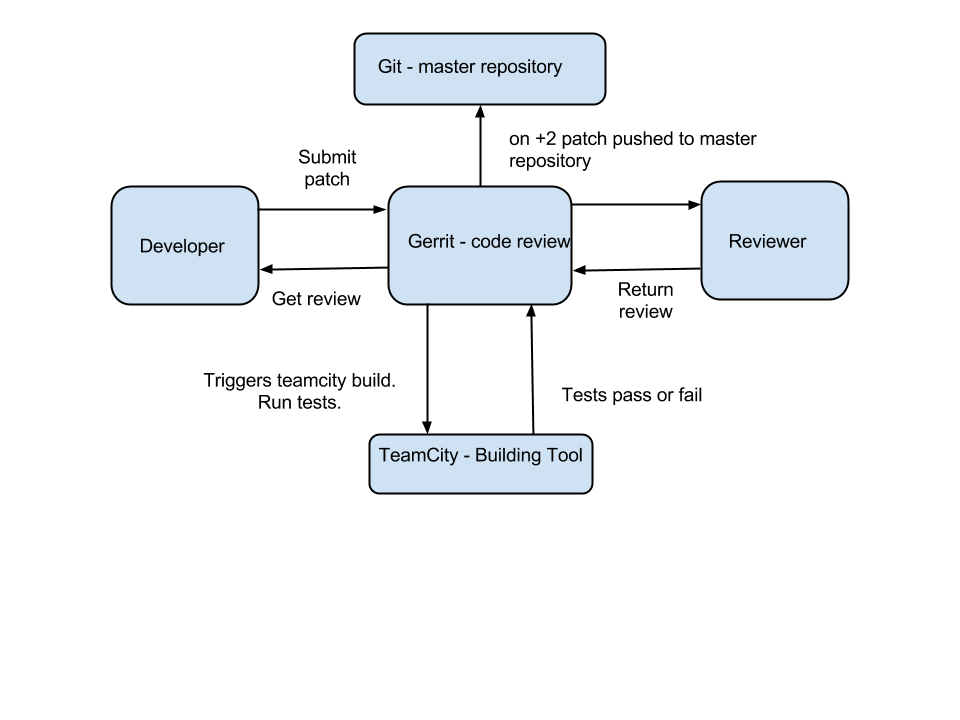
\includegraphics[width=0.75\textwidth]{gerrit1.png}
      \caption{Gerrit structure}
    \end{figure}
  Code review helps team members to follow similar code conventions, 
  keep code clean and readable and find bugs. Also code review helps developers to know more about 
  the whole project they are working in. Integrating Gerrit with an automated build tool, 
  such as TeamCity, allows to run tests before publishing commit for review. 
  The patch with failing tests is rejected automatically and an email with report for all failing tests sended 
  to the author of the patch. As an overall code review helps to keep source code quality on a higher level.


  \subsection{Testbench class diagram}
  
  \section{Example}

  
  The hierarchy of classes in testbench consists of many tens of classes and each class has tens of methods.
  Here we will describe the most important classes and the basic principles.

    \includegraphics{class.1}
    
AbstractHasTestBenchCommandExecutor class provides  `\$(Class clazz)' and
`\$\$(Class clazz)' methods which create a query for searching elements of
the given type.
 `\$' method builds a recursive search query and `\$\$' a non-recursive one.
 Non-recursive search query looks only for direct children of the element, while it’s recursive analog looks
  through all children of the element. Children elements are inner html-elements.
   For example if web-page has the following DOM(Document-Object Model). 
   Button and checkbox input elements are children elements of the div element with id id1.
  \lstset{language=HTML}
    \begin{lstlisting}
      <div id=”id1”>
        <input type="button">
        <input type ="checkbox">
      </div>
  \end{lstlisting}
  
  
ElementQuery<T> used for locating web elements(vaadin buttons, text fields, labels, etc.) on the web-page.
 Generic parameter T specifies the type of a searched element. 
 ElementQuery class provides methods for searching the element based on element’s id,class,
  caption or other criteria. These methods can be considered as filters in the query.
   ElementQuery uses the Builder pattern, which helps to add several filters to build a specific query and after
    the query is built execute it.

For example to find all children elements which are buttons:
  \lstset{language=Java}
    \begin{lstlisting}
    AbstractHasTestBenchCommandExecutor elem = getParentElement();
    List<Button> allButtons=elem.$(ButtonElement.class).all();
  \end{lstlisting}
  
To restrict search for buttons with caption “ok” we add a caption filter to the query.
  \lstset{language=Java}
  \begin{lstlisting}
  AbstractHasTestBenchCommandExecutor elem = getParentElement();
  List<Button> allButtons=elem.$(ButtonElement.class).caption(“ok”).all();
  \end{lstlisting}
  
TestbenchElemenet - is a base class for operating vaadin components. In includes methods to access properties common to all Vaadin elements, such as getSize(), getLocation(), getCssValue(), etc. TestbenchElement class uses Selenium WebElement class as a foundation and extend it’s functionality by using JavascriptExecutor, which allows to execute JavaScript code, and change the default element behaviour. 

ButtonElement, MenuBarElement, TableElement, etc. - implement specific class features. The default naming conventions is Vaadin component name + “Element”. In other words ButtonElement accesses buttons methods, TableElement table methods and so on. The important aspect is that hierarchy of testbench elements is similar to vaadin elements. That gives more flexibility when writing tests. Let’s look at the example:

The  developer/tester can specify concrete class for getting access to specific methods of the element:
 
 \lstset{language=Java}
  \begin{lstlisting}
  TableElement table= getElement();.$(TableElement.class).first();
  TableRowElement row=table.getRow(0);
 \end{lstlisting}
or use a more generic class to utilize method of a parent class, for example get caption of all elements :

  \lstset{language=Java}
  \begin{lstlisting}
  List<TestBenchElement> elements= getElement().$(TestBenchElement.class).all();
  List<String captions=new ArrayList<String ();
    for(int i =0;i<elements.size();i++) {
      captions.add(elements.get(i).getCaption());
    }
  }
  \end{lstlisting}

\subscection {Basic test case structure}
To use TestBench, the test case class should extend the TestBenchTestCase class,
which provides the WebDriver and ElementQuery APIs. A developer
can configure Testbench test by using following annotations:
\begin{itemize}
  \item \@Rule -defines certain TestBench parameters.
  \item \@Before - the annotated method is executed before each test.
  \item \@Test - annotates the tested method.
  \item \@After - the annotated method is executed after test.
\end{itemize}

A typical test case structure is the is the following:
\begin{itemize}
  \item Set TestBench parameters.
  \item Open the tested web-page URL.
  \item Find an element for interraction (Button, TextField).
  \item Interact with the elements (click buttons,menus,etc.).
  \item Find an element to check.
  \item Get and the value of the checked element.
  \item (optional) get screenshot.
\end{itemize}
	\lstset{language=Java}
	\begin{lstlisting}
		@Theme("mytheme")
		@Widgetset("com.example.testbench.MyAppWidgetset")
		public class MyUI extends UI {
		    @Override
		    protected void init(VaadinRequest vaadinRequest) {
		        final VerticalLayout layout = new VerticalLayout();
		        layout.setMargin(true);
		        setContent(layout);
		
		        Button button = new Button("Click Me");
		        button.addClickListener(new Button.ClickListener() {
		            @Override
		            public void buttonClick(ClickEvent event) {
		                layout.addComponent(new Label("Thank you for clicking"));
		            }
		        });
		        layout.addComponent(button);
		
		    }
		
		    @WebServlet(urlPatterns = "/*", name = "MyUIServlet", asyncSupported = true)
		    @VaadinServletConfiguration(ui = MyUI.class, productionMode = false)
		    public static class MyUIServlet extends VaadinServlet {
		    }
		}
	\end{lstlisting}
	\lstset{language=Java}
	\begin{lstlisting}
	public class ButtonTest extends TestBenchTestCase {
	    public static final String baseUrl = "http://localhost:8080";
	
	    @Before
	    public void setUp() throws Exception {
	        // Set WebDriver
	        setDriver(new FirefoxDriver());
	    }
	
	    @After
	    public void tearDown() throws Exception {
	        getDriver().quit();
	    }
	
	    @Test
	    public void testClick() {
	    	//Open URL
	        getDriver().get(baseUrl + "?restartApplication");
	        ButtonElement button = $(ButtonElement.class).first();
	        button.click();
	        LabelElement label = $(LabelElement.class).first();
	        String text = label.getText();
	        Assert.assertEquals("Thank you for clicking", text);
	    }
	}
	\end{lstlisting}
	
	When running this test you will get the following results:
\subsection {Challenges}
Because Vaadin is a statefull framework this brings additional complexity in
testing client-side and server-side communications. When event happens on the client side 
it will notify the server side. If this event affects the server side state, the
server side will notify the client side about this change.
 Because of a network delay or long time code execution on the server side there might be a delay between 
 client side action and the change on a client.  
 In these circumstances the client-side should wait for server side code to execute,
  because it might affect the next client side instruction.
  To handle this situation Testbench has waitForVaadin method, which suspend code execution until 
  there is no work to be done on the client side.
      
  
    \lstset{language=Java}
    \begin{lstlisting}
      public class TestUI extends UI{
        @Override
        protected void init(VaadinRequest request) {
          createUI();
        }
        public void createUI() {
          //step 1 
          TextField field1=new TextField();
          TextField field2=new TextField2;
          field1.setCaption("field1");
          field2.setCaption("field2");
          
          //step 2
          field1.addValueChangeListener(e->{
            field2.setValue("foo");
          });
        }
      }
    \end{lstlisting}  
    
    \lstset{language=Java}
    \begin{lstlisting}
      public class TextFieldSetValueTest extends TestBenchTestCase{
        @Test
        protected void testSetValue() {
          //Step 3
          TextFieldElement field1 =
            $(TextFieldElement.class).caption("field1).first();
            
          TextFieldElement field2 =
            $(TextFieldElement.class).caption("field2).first();  
          field1.setValue("bar");
          //Step 4
          waitForVaadin();
          
          //Step 5
          Assert.assertEquals(field2.getValue(), "foo");           
        }
      }
    \end{lstlisting}  
     \subsection {What was actually done}
      So here I will mention what was actually done during Testbench4
      development process, there were 3 people working on the project for 2-3
      months. Part of the work was a bit routine, like implementing some basic
      API or fixing bugs, but I think I can find some topics which interesting
      and new/have academic value. I don't want to dig deep into details, like
      why you can not confirm editing the textfield by sending a 'Return' code.
      But describe more the methodology and approaches used.